%\documentclass[journal,12pt,twocolumn]{IEEEtran}
%\newcommand{\myvec}[1]{\ensuremath{\begin{pmatrix}#1\end{pmatrix}}}
%\usepackage{lipsum} 
%\usepackage{amsmath}
%\usepackage[export]{adjustbox}
%\usepackage{bm}
%\usepackage{longtable}
%\usepackage[shortlabels]{enumitem}
%\usepackage{amssymb}
%\usepackage{mathtools}
%\usepackage[breaklinks=true]{hyperref}
%\usepackage{listings}
%\usepackage{color}                                            %%
%\usepackage{array}
%\usepackage{calc}       %%
%\usepackage{multirow}                                         %%
%\usepackage{hhline}                                           %%
%\usepackage{ifthen}                                           %%
%\usepackage{lscape}     
%\usepackage{multicol}
%\usepackage{tfrupee}
%% \usepackage{enumerate}
%\DeclareMathOperator*{\Res}{Res}
%\renewcommand\thesection{\arabic{section}}
%\renewcommand\thesubsection{\thesection.\arabic{subsection}}
%\renewcommand\thesubsubsection{\thesubsection.\arabic{subsubsection}}
%\renewcommand\thesectiondis{\arabic{section}}
%\renewcommand\thesubsectiondis{\thesectiondis.\arabic{subsection}}
%\renewcommand\thesubsubsectiondis{\thesubsectiondis.\arabic{subsubsection}}
%\newcommand{\uvec}[1]{\boldsymbol{\hat{\textbf{#1}}}}
%\hyphenation{op-tical net-works semi-conduc-tor}
%\def\inputGnumericTable{}  %%

%\graphicspath{ {./} }
%\usepackage{multicol}
%\usepackage{enumitem}
%\setlength{\columnsep}{1cm}
%\title{10th CBSE MATHEMATICS}
%\author{2020-21}
%\begin{document}
%
%\maketitle
%\newpage
%\bigskip






\let\negmedspace\undefined
\let\negthickspace\undefined
%\RequirePackage{amsmath}
\documentclass[journal,12pt,onecolumn]{IEEEtran}


%
% \usepackage{setspace}
%\usepackage{graphicx}
\usepackage{gensymb}
%\doublespacing
%\singlespacing
%\usepackage{silence}
%Disable all warnings issued by latex starting with "You have..."
%\usepackage{graphicx}
\usepackage{amssymb}
%\usepackage{relsize}
\usepackage[cmex10]{amsmath}
%\usepackage{amsthm}
%\interdisplaylinepenalty=2500
%\savesymbol{iint}
%\usepackage{txfonts}
%\restoresymbol{TXF}{iint}
%\usepackage{wasysym}
\usepackage{amsthm}
%\usepackage{pifont}
%\usepackage{iithtlc}
% \usepackage{mathrsfs}
% \usepackage{txfonts}
 \usepackage{stfloats}
% \usepackage{steinmetz}
 \usepackage{bm}
% \usepackage{cite}
% \usepackage{cases}
% \usepackage{subfig}
%\usepackage{xtab}
\usepackage{longtable}
%\usepackage{multirow}
%\usepackage{algorithm}
%\usepackage{algpseudocode}
\usepackage{enumitem}
 \usepackage{mathtools}
 \usepackage{tikz}
% \usepackage{circuitikz}
% \usepackage{verbatim}
%\usepackage{tfrupee}
\usepackage[breaklinks=true]{hyperref}
%\usepackage{stmaryrd}
%\usepackage{tkz-euclide} % loads  TikZ and tkz-base
%\usetkzobj{all}
\usepackage{listings}
    \usepackage{color}                                            %%
    \usepackage{array}                                            %%
    \usepackage{longtable}                                        %%
    \usepackage{calc}                                             %%
    \usepackage{multirow}                                         %%
    \usepackage{hhline}                                           %%
    \usepackage{ifthen}                                           %%
  %optionally (for landscape tables embedded in another document): %%
    \usepackage{lscape}     
% \usepackage{multicol}

%\usepackage{enumerate}

\usepackage{caption}
%\usepackage{wasysym}
%\newcounter{MYtempeqncnt}
\DeclareMathOperator*{\Res}{Res}
\DeclareMathOperator*{\equals}{=}
%\renewcommand{\baselinestretch}{2}
\renewcommand\thesection{\arabic{section}}
\renewcommand\thesubsection{\thesection.\arabic{subsection}}
\renewcommand\thesubsubsection{\thesubsection.\arabic{subsubsection}}

\renewcommand\thesectiondis{\arabic{section}}
\renewcommand\thesubsectiondis{\thesectiondis.\arabic{subsection}}
\renewcommand\thesubsubsectiondis{\thesubsectiondis.\arabic{subsubsection}}

% correct bad hyphenation here
\hyphenation{op-tical net-works semi-conduc-tor}
\def\inputGnumericTable{}                                 %%

\lstset{
%language=C,
frame=single, 
breaklines=true,
columns=fullflexible
}
%\lstset{
%language=tex,
%frame=single, 
%breaklines=true
%}



\begin{document}

%


\newtheorem{theorem}{Theorem}[section]
\newtheorem{problem}{Problem}
\newtheorem{proposition}{Proposition}[section]
\newtheorem{lemma}{Lemma}[section]
\newtheorem{corollary}[theorem]{Corollary}
\newtheorem{example}{Example}[section]
\newtheorem{definition}[problem]{Definition}
%\newtheorem{thm}{Theorem}[section] 
%\newtheorem{defn}[thm]{Definition}
%\newtheorem{algorithm}{Algorithm}[section]
%\newtheorem{cor}{Corollary}
\newcommand{\BEQA}{\begin{eqnarray}}
\newcommand{\EEQA}{\end{eqnarray}}
\newcommand{\define}{\stackrel{\triangle}{=}}
\newcommand*\circled[1]{\tikz[baseline=(char.base)]{
    \node[shape=circle,draw,inner sep=2pt] (char) {#1};}}
\bibliographystyle{IEEEtran}
%\bibliographystyle{ieeetr}


\providecommand{\mbf}{\mathbf}
\providecommand{\pr}[1]{\ensuremath{\Pr\left(#1\right)}}
\providecommand{\qfunc}[1]{\ensuremath{Q\left(#1\right)}}
\providecommand{\sbrak}[1]{\ensuremath{{}\left[#1\right]}}
\providecommand{\lsbrak}[1]{\ensuremath{{}\left[#1\right.}}
\providecommand{\rsbrak}[1]{\ensuremath{{}\left.#1\right]}}
\providecommand{\brak}[1]{\ensuremath{\left(#1\right)}}
\providecommand{\lbrak}[1]{\ensuremath{\left(#1\right.}}
\providecommand{\rbrak}[1]{\ensuremath{\left.#1\right)}}
\providecommand{\cbrak}[1]{\ensuremath{\left\{#1\right\}}}
\providecommand{\lcbrak}[1]{\ensuremath{\left\{#1\right.}}
\providecommand{\rcbrak}[1]{\ensuremath{\left.#1\right\}}}
\theoremstyle{remark}
\newtheorem{rem}{Remark}
\newcommand{\sgn}{\mathop{\mathrm{sgn}}}
\providecommand{\abs}[1]{\left\vert#1\right\vert}
\providecommand{\res}[1]{\Res\displaylimits_{#1}} 
\providecommand{\norm}[1]{\left\lVert#1\right\rVert}
%\providecommand{\norm}[1]{\lVert#1\rVert}
\providecommand{\mtx}[1]{\mathbf{#1}}
\providecommand{\mean}[1]{E\left[ #1 \right]}
\providecommand{\fourier}{\overset{\mathcal{F}}{ \rightleftharpoons}}
%\providecommand{\hilbert}{\overset{\mathcal{H}}{ \rightleftharpoons}}
\providecommand{\system}{\overset{\mathcal{H}}{ \longleftrightarrow}}
	%\newcommand{\solution}[2]{\textbf{Solution:}{#1}}
\newcommand{\solution}{\noindent \textbf{Solution: }}
\newcommand{\cosec}{\,\text{cosec}\,}
\providecommand{\dec}[2]{\ensuremath{\overset{#1}{\underset{#2}{\gtrless}}}}
\newcommand{\myvec}[1]{\ensuremath{\begin{pmatrix}#1\end{pmatrix}}}
\newcommand{\mydet}[1]{\ensuremath{\begin{vmatrix}#1\end{vmatrix}}}
%\numberwithin{equation}{section}
%\numberwithin{equation}{subsection}
%\numberwithin{problem}{section}
%\numberwithin{definition}{section}
\makeatletter
\@addtoreset{figure}{problem}
\makeatother



\let\StandardTheFigure\thefigure
\let\vec\mathbf
%\renewcommand{\thefigure}{\theproblem.\arabic{figure}}
%\renewcommand{\thefigure}{\theproblem}
%\setlist[enumerate,1]{before=\renewcommand\theequation{\theenumi.\arabic{equation}}
%\counterwithin{equation}{enumi}


%\renewcommand{\theequation}{\arabic{subsection}.\arabic{equation}}

\def\putbox#1#2#3{\makebox[0in][l]{\makebox[#1][l]{}\raisebox{\baselineskip}[0in][0in]{\raisebox{#2}[0in][0in]{#3}}}}
     \def\rightbox#1{\makebox[0in][r]{#1}}
     \def\centbox#1{\makebox[0in]{#1}}
     \def\topbox#1{\raisebox{-\baselineskip}[0in][0in]{#1}}
     \def\midbox#1{\raisebox{-0.5\baselineskip}[0in][0in]{#1}}

\vspace{3cm}

\title{
	%\logo{
%Computational Approach to School Geometry
	\textbf{  $10^{th}$ CBSE Mathematics Paper - 2022}
%	}
}
\author{ G V V Sharma$^{*}$% <-this % stops a space
	\thanks{*The author is with the Department
		of Electrical Engineering, Indian Institute of Technology, Hyderabad
		502285 India e-mail:  gadepall@iith.ac.in. All content in this manual is released under GNU GPL.  Free and open source.}
	
}	
%\title{
%	\logo{Matrix Analysis through Octave}{\begin{center}\includegraphics[scale=.24]{tlc}\end{center}}{}{HAMDSP}
%}


% paper title
% can use linebreaks \\ within to get better formatting as desired
%\title{Matrix Analysis through Octave}
%
%
% author names and IEEE memberships
% note positions of commas and nonbreaking spaces ( ~ ) LaTeX will not break
% a structure at a ~ so this keeps an author's name from being broken across
% two lines.
% use \thanks{} to gain access to the first footnote area
% a separate \thanks must be used for each paragraph as LaTeX2e's \thanks
% was not built to handle multiple paragraphs
%

%\author{<-this % stops a space
%\thanks{}}
%}
% note the % following the last \IEEEmembership and also \thanks - 
% these prevent an unwanted space from occurring between the last author name
% and the end of the author line. i.e., if you had this:
% 
% \author{....lastname \thanks{...} \thanks{...} }
%                     ^------------^------------^----Do not want these spaces!
%
% a space would be appended to the last name and could cause every name on that
% line to be shifted left slightly. This is one of those "LaTeX things". For
% instance, "\textbf{A} \textbf{B}" will typeset as "A B" not "AB". To get
% "AB" then you have to do: "\textbf{A}\textbf{B}"
% \thanks is no different in this regard, so shield the last } of each \thanks
% that ends a line with a % and do not let a space in before the next \thanks.
% Spaces after \IEEEmembership other than the last one are OK (and needed) as
% you are supposed to have spaces between the names. For what it is worth,
% this is a minor point as most people would not even notice if the said evil
% space somehow managed to creep in.

%\WarningFilter{latex}{LaTeX Warning: You have requested, on input line 117, version}


% The paper headers
%\markboth{Journal of \LaTeX\ Class Files,~Vol.~6, No.~1, January~2007}%
%{Shell \MakeLowercase{\textit{et al.}}: Bare Demo of IEEEtran.cls for Journals}
% The only time the second header will appear is for the odd numbered pages
% after the title page when using the twoside option.
% 
% *** Note that you probably will NOT want to include the author's ***
% *** name in the headers of peer review papers.                   ***
% You can use \ifCLASSOPTIONpeerreview for conditional compilation here if
% you desire.




% If you want to put a publisher's ID mark on the page you can do it like
% this:
%\IEEEpubid{0000--0000/00\$00.00~\copyright~2007 IEEE}
% Remember, if you use this you must call \IEEEpubidadjcol in the second
% column for its text to clear the IEEEpubid mark.



% make the title area
\maketitle


\bigskip

%\renewcommand{\thefigure}{\theenumi}
\renewcommand{\thetable}{\theenumi}
\renewcommand{\theequation}{\theenumi}

%\begin{abstract}
%%\boldmath
%In this letter, an algorithm for evaluating the exact analytical bit error rate  (BER)  for the piecewise linear (PL) combiner for  multiple relays is presented. Previous results were available only for upto three relays. The algorithm is unique in the sense that  the actual mathematical expressions, that are prohibitively large, need not be explicitly obtained. The diversity gain due to multiple relays is shown through plots of the analytical BER, well supported by simulations. 
%
%\end{abstract}
% IEEEtran.cls defaults to using nonbold math in the Abstract.
% This preserves the distinction between vectors and scalars. However,
% if the journal you are submitting to favors bold math in the abstract,
% then you can use LaTeX's standard command \boldmath at the very start
% of the abstract to achieve this. Many IEEE journals frown on math
% in the abstract anyway.

% Note that keywords are not normally used for peerreview papers.
%\begin{IEEEkeywords}
%Cooperative diversity, decode and forward, piecewise linear
%\end{IEEEkeywords}



% For peer review papers, you can put extra information on the cover
% page as needed:
% \ifCLASSOPTIONpeerreview
% \begin{center} \bfseries EDICS Category: 3-BBND \end{center}
% \fi
%
% For peerreview papers, this IEEEtran command inserts a page break and
% creates the second title. It will be ignored for other modes.
%\IEEEpeerreviewmaketitle

%\begin{abstract}
%This manual provides an introduction to vectors and their properties,  %based on the question papers, year 2020,  from Class 10 and 12, CBSE; JEE %and JNTU.  
%\end{abstract}
%


\section{\textbf{Section-A}}
\begin{enumerate}[\arabic*]

\item     
 \begin{enumerate}
  \item In Fig $\ref{Fig1}$, $\Vec{AB}$ is diameter of a circle centred at O. $\Vec{BC}$ is the tangent to the circle at B. If $\Vec{OP}$ bisects the chord $\Vec{AD}$ and  $\angle{AOP} = 60^\circ$, then find m$\angle{C}$.


   \begin{figure}[h!]
     \centering
     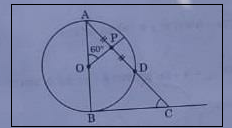
\includegraphics[width=0.4\columnwidth]{Fig1.png}
	 \caption{}
	 \label{Fig1}
	 
    \end{figure}

   \item In Fig $\ref{Fig2}$, $\Vec{XAY}$ is a tangent to the circle centred at O. If $\angle{ABO} = 40^\circ$, then find m$\angle{BAY}$ and m$\angle{AOB}$.


    \begin{figure}[h!]
     \centering
     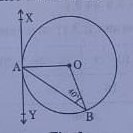
\includegraphics[width=0.4\columnwidth]{Fig2.png}
	 \caption{}
	 \label{Fig2}
    \end{figure}

\end{enumerate}

\item If mode of the following frequency distribution is 55, then find the value of x. \\
     \vspace{2mm}\\
     \scalebox{0.7}{
     \begin{tabular}{|l|c|c|c|c|c|c|}
      \hline
      Class : & 0-15 & 15-30 & 30-45 & 45-60 & 60-75 & 75-90  \\
      \hline
      Frequency :  & 10 & 7 & x & 15 & 10 & 12\\
      \hline
     \end{tabular}
     }
     \vspace{5mm} \\
     

\item 
\begin{enumerate} 
   \item In an A.P,  if the sum of third and seventh term is zero, find its $5^{th}$ term. \\

   \vspace{3mm} \\

   \begin{center}
     \textbf{OR}
   \end{center}

   \item Determine the A.P. whose third term is 5 and seventh term is 9.\\

\end{enumerate}

\item Solve the quadratic equation $x^2+2\sqrt{2}x-6 = 0$.\\


\item Find the sum of the first 20 terms of an A.P. whose $n^{th}$ term is given as $a_{n}$ = 5-2n \\


\item A solid piece of metal in the form of a cuboid of dimensions 11 cm x 7 cm x 7 cm is melted to form \textbf{n} number of solid spheres of radii $\frac {7}{2}$ cm each. Find the value of \textbf{n}. \\

\section{\textbf{Section-B}}

\item 
\begin{enumerate}   
   \item The mean of the following frequency distribution is 25. Find the value of f. \\
     \vspace{2mm}\\
     \scalebox{0.7}{
     \begin{tabular}{|l|c|c|c|c|c|}
      \hline
      Class : & 0-10 & 10-20 & 20-30 & 30-40 & 40-50 \\
      \hline
      Frequency :  & 5 & 18 & 15 & f & 6 \\
      \hline
     \end{tabular}
     } 
     \vspace{3mm}\\ 
                      \begin{center}
                      \textbf{OR}
                      \end{center}
     \vspace{5mm}\\
     
    \item Find the mean of the following frequency data using assumed mean methid. \\
     \vspace{2mm}\\
     \scalebox{0.7}{
     \begin{tabular}{|l|c|c|c|c|c|}
      \hline
      Class : & 0-5 & 5-10 & 10-15 & 15-20 & 20-25 \\
      \hline
      Frequency :  & 8 & 7 & 10 & 13 & 12 \\
      \hline
     \end{tabular}
     }
     \vspace{5mm} \\  
      
\end{enumerate}
    
\item From a point on a bridge across a river, the angles of depression of the banks on opposite sides of the river are $30^\circ$ and $45^\circ$. If the bridge is at a height of 8m from the banks, then find the width of the river.
    
    Refer Fig $\ref{Fig3}$
    
    
    \begin{figure}[h!]
        \centering
        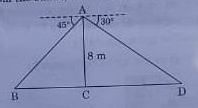
\includegraphics[width=0.4\columnwidth]{Fig3.png}
    	\caption{}
    	\label{Fig3}
     \end{figure}
     \vspace{5mm}\\
     
      
\item Heights of 50 students of class X of a school are recorded and following data is obtained:\\
     \vspace{2mm}\\
     \scalebox{0.7}{
     \begin{tabular}{|l|c|c|c|c|c|c|}
        \hline
        Height (in cm) : & 130-135 & 135-140 & 140-145 & 145-150 & 150-155 & 155-160  \\
        \hline
        Number of Students:  & 4 & 11 & 12 & 7 & 10 & 6\\
        \hline
     \end{tabular}
     }
     \vspace{3mm} \\
     Find median height of the students.
     \vspace{2mm} \\
     
\item Construct a pair of tangents to a circle of radius 4 cm from a point \textbf{P} lying outside the circel at a distance of 6 cm from the centre. \\


     
\section{\textbf{Section C}}
   
\item
    \begin{enumerate}
    
    \item A 2-digit number is such that the product of its digits is 24. if 18 is subtracted from the number, the digits interchange their places. Find the number. \\
    
\begin{center}
   \textbf{OR}
\end{center}

    \vspace{2mm} \\
    
    \item The difference of the squares of two numbers is 180. The square of the smaller number is 8 times the greater number. Find the two numbers. \\
    
\end{enumerate}
    
\item Prove that a parallelogram circumscribing a circle is a rhombus.\\

\item \textbf{Case Study-1}: \\
        
        
 \textbf{Kite Festival} 
        
        Kite festival is celebrated in many countries at different times of the year. In India, every year, $14^{th}$ January is celebrated as International Kite Day. On this day, many people visit India and participate in the festival by flying various kinds of kite. 
        The picture given below, three kites flying together.
        
        \begin{figure}[h!]
        \centering
        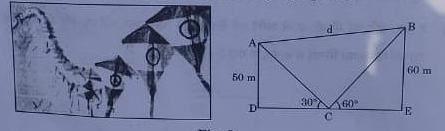
\includegraphics[width=0.8\columnwidth]{Fig4.png}
    	\caption{}
    	\label{Fig4}
     \end{figure} 
        
        
        In Fig $\ref{Fig4}$, the angle of elevation of two kites (Points A and B) from the hands of a man (Point C) are found to be $30^\circ$ and $60^\circ$ respectively. Taking $Vec{AD}$ = 50 m and $Vec{BE}$ = 60 m, find \\
        
        (1) the lenghts of strings used (take them straight) for kites A and B as shown in the figure.\\
        
        
        (2) the distnce 'd' between these two kites. \\
   
   
\item \textbf{Case Study-2}: \\  
   
      
          A circus is a company of performers who put on shows of acrobats, clowns etc to entertain people started around 250 years back, in open fields, now generally performed in tents. \\
          
          
          One such circus tent is shown in Fig $\ref{Fig5}$.   \\
          
          
     
     The tent is in the shape of a cylinder surmounted by a conical top. If the height and diameter of the cylindrical part are 9 m and 30 m respectively and height of the conical part is 8 m with same diameter as that of the cylindrical part, then find \\
     
     (1) the area of the canvas used in the tent. \\
     (2) the cost of the canvas bought for the tent at the rate 200 rupees          per sq m, if 30 sq m canvas wasted during the stitching. \\
     
     \begin{figure}[h!]
       \centering
        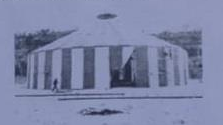
\includegraphics[width=0.8\columnwidth]{Fig5.png}
    	\caption{}
    	\label{Fig5}
     \end{figure} 
        
    \end{enumerate}
    
\end{document}
